\documentclass{beamer}
\usetheme{Madrid}

% escreve textos gerados em portugues
\usepackage[brazilian]{babel}
% aceita unicode
\usepackage[utf8]{inputenc}

\author[Andre Esteve and Zhenlei Ji]{
Andre Petris Esteve - \texttt{andreesteve@gmail.com}\\
Zhenlei Ji - \texttt{zhenlei.ji@gmail.com}}
\institute[IC\textbackslash UNICAMP]{
MC806 - Operational System Topics\\}

\title[Linux VFS]{Linux Virtual File System}
\subtitle[]{The linux VFS and FUSE - Filesystem in User Space}

\date[10/20/2011]{October 20th, 2011}

\begin{document}

%--- create section frame for every new section --%
\AtBeginSection[]
{
   \begin{frame}[shrink=0.7]
       \frametitle{Agenda}
       \tableofcontents[currentsection]
   \end{frame}
}

\begin{frame}[plain]
  \titlepage
\end{frame}

%--- content -------------------------------------%
\begin{frame}{Agenda}
  \tableofcontents[hidesubsections]
\end{frame}

\section{Objectives}

\begin{frame}{Objectives}

  \begin{block}{What do we want?}

	\begin{itemize}[<+->]

		\item{View the Linux's Virtual Filesystem as a series of object oriented entities (classes and objects)}\footnotemark

		\item{Construct UML models to easy understanding}
		
		\item{Provide initial information so one can start developing a filesystem module for the Linux kernel}
	
	\end{itemize}

  \end{block}

	\footnotetext[1]{Althought the linux kernel is written in C, it's possible to profit from some object oriented features through programming tricks. For further deailts see: OOC, Axel Schreiner}

\end{frame}

\begin{frame}{Warning}

  \begin{block}{Please note!}

	\begin{itemize}[<+->]

		\item{All information here is based extensively on linux kernel 3.1-rc8 source code\footnotemark[1]}

		\item{Some models are represented at a certain level of abstraction and may omit some implementation information}
	
	\end{itemize}

  \end{block}

	\footnotetext[1]{You can easly find something in the kernel source code using this tools: http://lxr.linux.no/linux}

\end{frame}

\section{Overview}

\begin{frame}{What's Linux's Virtual Filesystem}

  \begin{block}{Definition}

	The Virtual File System (also known as the Virtual Filesystem Switch)
	is the software layer in the kernel that provides the filesystem
	interface to userspace programs. It also provides an abstraction
	within the kernel which allows different filesystem implementations to
	coexist. \footnotemark[1]

  \end{block}

	\footnotetext[1]{Overview of the Linux Virtual File System, Richard Gooch, from Linux "documentation"}

\end{frame}

\begin{frame}{Linux's Virtual Filesystem Overview}

	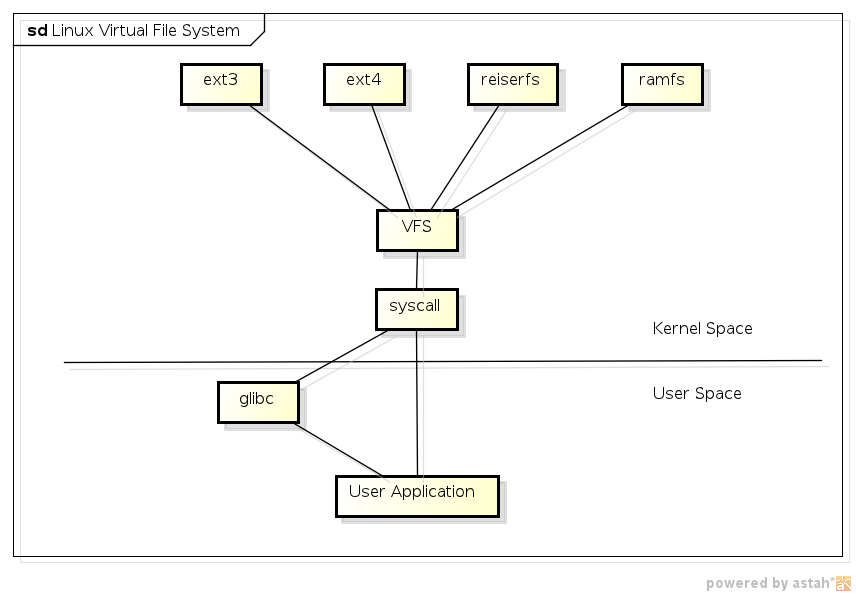
\includegraphics[scale=0.5]{img/vfs_overview.png}

\end{frame}

\begin{frame}{Linux's Virtual Filesystem Overview}

	\begin{itemize}[<+->]
	
		\item[$\bullet$]{Abstraction layer to allow different fs\footnotemark[1] to coexist}	
		\item[$\bullet$]{Only point of access to fs calls}
		\item[$\bullet$]{Implements common fs operations}
			\begin{itemize}
				\item[$-$]{Common inicialization operations}
				\item[$-$]{Mounting (at a certain level) and managing mount points}
				\item[$-$]{Path lookup}
				\item[$-$]{Caching}
			\end{itemize}	
	\end{itemize}

	\footnotetext[1]{Short for "filesystem"}

\end{frame}

\begin{frame}{Linux's Virtual Filesystem Overview}

	\begin{block}{How is a filesystem implemented?}
		With loadable kernel modules\footnotemark[1] (LKM), or just modules for short.
	\end{block}

	\vspace{15pt}
	
	\pause

	\begin{itemize}[<+->]
	
		\item[$\bullet$]{It's possible to compile a LKM with the base kernel}
		\item[$\bullet$]{Or just load the LKM during system usage}

	\end{itemize}

	\footnotetext[1]{For an extensive discussion about LKM, see: \texttt{http://www.tldp.org/HOWTO/Module-HOWTO/}}

\end{frame}

%--- Linux's Virtual File System Core Elements------------------%

\section{Core Elements}

\begin{frame}{Linux's Virtual Filesystem Core Elements}

	\begin{description}[<+->]\itemsep4pt
			
		\item[file\_system\_type]{Information about a specific fs type}
		\item[vfsmount]{Mount point information}		
		\item[super\_block]{Represents a mounted filesystem}
		\item[inode]{Information about a file (on disk, memory or network)}
		\item[dentry]{A directory entry}
		\item[file]{A file abstraction - points to a inode}

		\vspace{15pt}

		\item{Note: Every element, except vfsmount, is defined at include/linux/fs.h.}

	\end{description}

\end{frame}

\begin{frame}{Linux's Virtual Filesystem Core Elements}
	
	\center{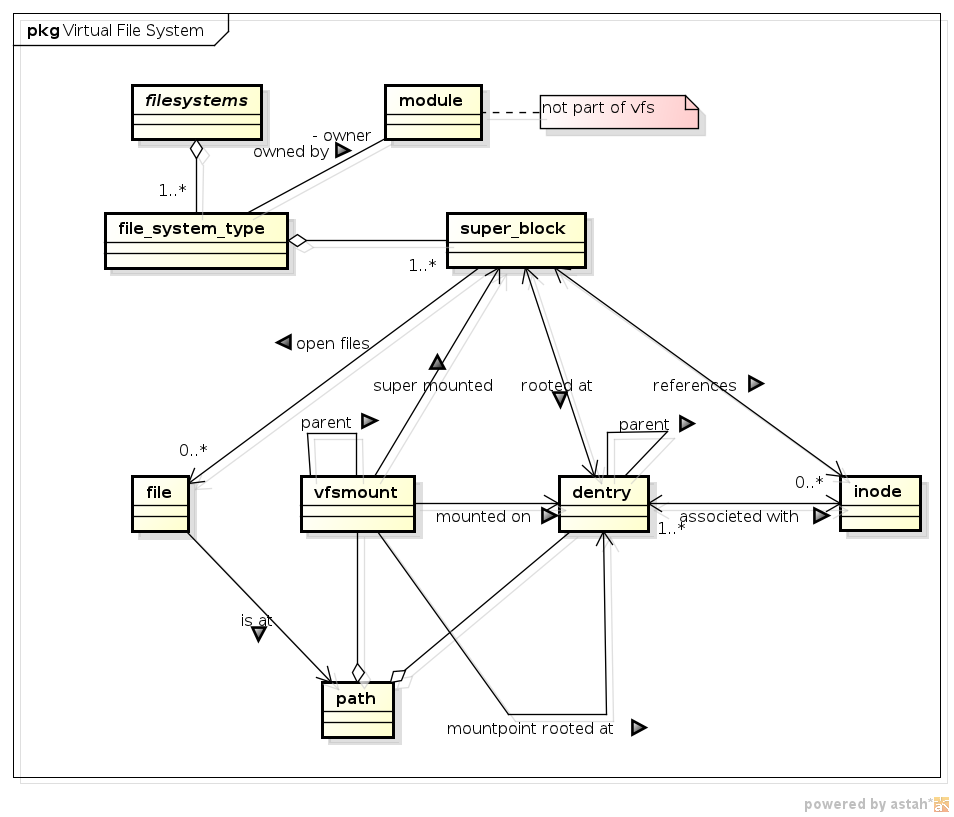
\includegraphics[scale=0.35]{img/vfs_elements_simple.png}}

\end{frame}

\subsection{file\_system\_type}

\begin{frame}{file\_system\_type}
	
	\center{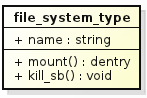
\includegraphics{img/file_system_type.png}}
	
\end{frame}

\begin{frame}{file\_system\_type}
	
	\begin{itemize}[<+->]
	
		\item[$\bullet$]{Represents a filesystem type (e.g. ext3, nfs, fuse)}
		\item[$\bullet$]{fs/filesystems.c has a linked list of filesystem types}
		\item[$\bullet$]{Each filesystem type must have a unique name}
		\item[$\bullet$]{Each filesystem type has a linked list of super blocks in use (i.e. mounted)}		
		\item[$\bullet$]{Each filesystem type is owned by a module (which implements it)}
		\item[$\bullet$]{Each filesystem type has a function to mount a (possibly new) instance of the filesystem}
		
	\end{itemize}

\end{frame}

\subsection{vfsmount}
	
\begin{frame}{vfsmount}
	
	\center{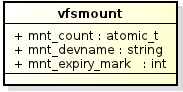
\includegraphics{img/vfsmount.png}}
	
\end{frame}

\begin{frame}{vfsmount}
	
	\begin{itemize}[<+->]

		\item[$\bullet$]{Defined at include/linux/mount.h}	

		\item[$\bullet$]{Store information about a mount point}
			\begin{itemize}
				\item[$-$]{Device name (if any)}
				\item[$-$]{Use count (if 0 the fs could be unmounted if mnt\_expiry\_mark is set) }
			\end{itemize}	
		
		\item[$\bullet$]{Refers to the parent mount point (the one its mounted on) and has a list of mounted children}
		\item[$\bullet$]{Points to the parent (mount point) dentry root}
		\item[$\bullet$]{Has a dentry for its own root}
		\item[$\bullet$]{Has the super block of the mounted filesystem}		
		\item[$\bullet$]{Not directly handled by a filesystem implementation}
		
	\end{itemize}

\end{frame}

\subsection{super\_block}

\begin{frame}{super\_block}
	
	\center{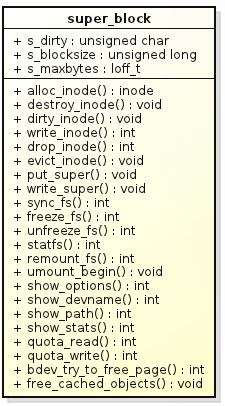
\includegraphics[scale=0.65]{img/super_block.png}}
	
\end{frame}

\begin{frame}{super\_block}
	
	\begin{itemize}[<+->]

		\item[$\bullet$]{Represents a filesystem instance}
		\item[$\bullet$]{When the filesystem is disk based, the super block usualy is persisted on disk}		
		\item[$\bullet$]{It's kept on memory, but there's a dirty flag so it can eventualy be flush to disk (for disk based fs)}
		\item[$\bullet$]{Defines filesystem's properties}
			\begin{itemize}
				\item[$-$]{block size}
				\item[$-$]{maximum file size}
				\item[$-$]{access time granularity, among others}
			\end{itemize}	
		
		\item[$\bullet$]{Refers to its filesystem type (and thus module owner)}
		\item[$\bullet$]{Points to its dentry root}
		\item[$\bullet$]{Has a dentry for its own root}
		\item[$\bullet$]{Has lists for open files and inodes in use}
		\item[$\bullet$]{Has functions to handle quota operations and inode manipulation}
		
	\end{itemize}

\end{frame}

\subsection{inode}
\begin{frame}{inode}
	
	\begin{itemize}[<+->]

		\item[$\bullet$]{Each object in the filesytem is represented by an inode}
		\item[$\bullet$]{Each inode is indentified by a unique inode number within the filesystem}		
		\item[$\bullet$]{The inode is only instantiated in memory at the time the file is opened}
		
		\item[$\bullet$]{Defines inode atributes}
			\begin{itemize}
				\item[$-$]{i\_ino}
				\item[$-$]{i\_blksize, i\_block, i\_bytes}
				\item[$-$]{i\_atime, i\_mtime, i\_ctime}
			\end{itemize}
	\end{itemize}

	\begin{itemize}[<+->]
		\item[$\bullet$]{Defines inode\_operations}
			\begin{itemize}
				\item[$-$]{create(dir, dentry, mode, nameidata)}
				\item[$-$]{lookup(dir, dentry, nameidata)}
				\item[$-$]{link(old\_dentry, dir, new\_dentry)}
				\item[$-$]{mkdir(dir, dentry, mode)}
				\item[$-$]{rmdir(dir, dentry)}
				\item[$-$]{rename(old\_dir, old\_dentry, new\_dir, new\_dentry)}	
				\item[$-$]{permission(inode, mask, nameidada)}
			\end{itemize}

		\item[$\bullet$]{A single inode can be pointed to by multiple dentries (hard links)}
	\end{itemize}
\end{frame}

\subsection{dentry}
\begin{frame}{dentry}
	
	\begin{itemize}[<+->]

		\item[$\bullet$]{The VFS considers each directory a file that contains a list of files and directories}
		\item[$\bullet$]{Once a directory entry is read into memory, it is tranformed by the VFS into a dentry object}
			\begin{itemize}
				\item[$-$]{Example: /tmp/tex \newline tmp and vi are files, both represented by the inode.}
			\end{itemize}
		\item[$\bullet$]{The concept of input directory (dentry)}
		\item[$\bullet$]{Specifc component of the path}
		\item[$\bullet$]{The VFS instantiate these object "on the fly" when you make operation on directories}
		\item[$\bullet$]{It's kept on memory}
	\end{itemize}

\end{frame}

\begin{frame}{dentry}
	
	\begin{itemize}[<+->]
		\item[$\bullet$]{Defines dentry atributes}
			\begin{itemize}
				\item[$-$]{d\_count}
				\item[$-$]{d\_inode}
				\item[$-$]{d\_parent}
				\item[$-$]{d\_name}
			\end{itemize}

		\item[$\bullet$]{Dentry States:}
			\begin{itemize}
				\item[$-$]{Free: no valid information and is not used}
				\item[$-$]{Unused: valid information and is not used, may be discarted if necessary}
				\item[$-$]{In use: valid information and is used, cannot be discarted}
				\item[$-$]{Negative: the inode associated with the dentry does not exist or invalid}
			\end{itemize}
	\end{itemize}

\end{frame}

%--- Dentry cache---------------------------------%

\section{Dentry cache}
	\begin{itemize}[<+->]
		\item[$\bullet$]{Reading a directory entry from disk and constructing the correponding dentry object requires considerable time}
		\item[$\bullet$]{A set of dentry in the in-use, unused, or negative state}
		\item[$\bullet$]{A hash table to derive the dentry object associated with a given filename and  given directory quickly}
		\item[$\bullet$]{}
		\item[$\bullet$]{}
			\begin{itemize}
				\item[$-$]{Example: /tmp/tex \newline tmp and vi are files, both represented by the inode.}
			\end{itemize}
		\item[$\bullet$]{}
	\end{itemize}

%--- Dentry cache---------------------------------%

\subsection{file}

\section{Hard link x Simbolic link}

\section{Operations detailed}

\subsection{Mount}

\begin{frame}{Mount activity diagram}
	
	\center{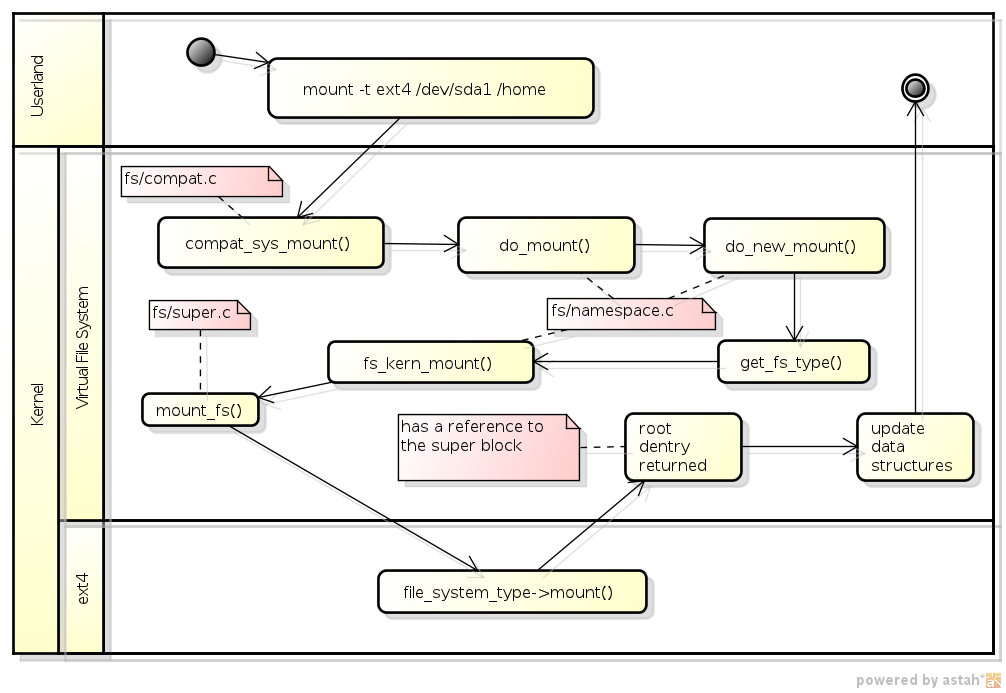
\includegraphics[scale=0.4]{img/mount_act.png}}
	
\end{frame}

\subsection{Read (a file)}

%--- FUSE ---------------------------------%

\section{Getting conFUSEed}

\subsection{What is FUSE?}

\begin{frame}{What is FUSE?}

	\begin{block}{Filesystem in User Space}

		\begin{itemize}[<+->]

			\item{An open source framework for implementing filesystem in user land}\footnotemark[1]
	
		\end{itemize}

	\end{block}

	\footnotetext[1]{http://fuse.sourceforge.net/}

\end{frame}

\begin{frame}{What is it good for?}

	\begin{itemize}[<+->]

		\item{Higher abstraction - it's easier to write a fuse-based filesystem than a "native" linux filesystem}

		\item{No kernel recompilation or module installs}
		
		\item{FUSE is already compiled within the kernel in common distros (e.g. Ubuntu)}
	
		\item{Applications in user space has lots of ready-to-use libraries}

		\item{Write your filesystem in any programming language}
		
		\item{You won't crash the system :)}
	
	\end{itemize}

\end{frame}

\begin{frame}{What is it NOT good for?}

	\begin{itemize}[<+->]

		\item{Performance penalty (switches between user and kernel modes and higher indirection level)}

		\item{If you need to override some kernel functionality (as the dentry cache, for instance)}
	
	\end{itemize}

\end{frame}

\begin{frame}{What is fuse-based?}

	\begin{itemize}[<+->]

		\item{Gmail filesystem}\footnotemark[1]
		
		\item{sshfs}\footnotemark[2]
		
		\item{WikipediaFS}\footnotemark[3]
	
	\end{itemize}
	
	\footnotetext[1]{http://richard.jones.name/google-hacks/gmail-filesystem/gmail-filesystem.html}

	\footnotetext[2]{http://fuse.sourceforge.net/sshfs.html}	

	\footnotetext[3]{http://en.wikipedia.org/wiki/WikipediaFS}	
	
\end{frame}

\subsection{FUSE Architecture}

\begin{frame}{FUSE basic workings}
	
	\center{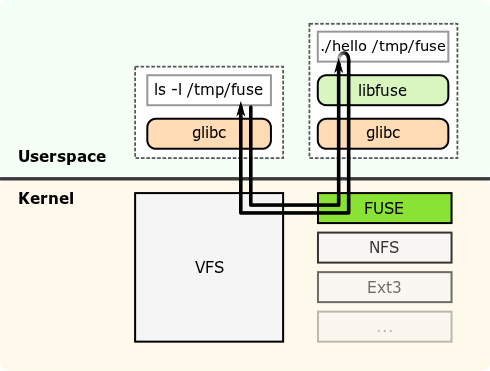
\includegraphics[scale=0.5]{img/fuse_structure.png}}
	
	\let\thefootnote\relax\footnotetext{Source: http://fuse.sourceforge.net/}
	
\end{frame}

\begin{frame}{FUSE in deep}
	
	\begin{itemize}[<+->]

		\item{FUSE is composed of two parts}
			\begin{itemize}
				\item[$-$]{User space library - libfuse - provies to the filesystem application an API}
				\item[$-$]{Kernel surrogate filesystem implementation - fs/fuse }
			\end{itemize}	
	
	\end{itemize}
	
\end{frame}

\begin{frame}{FUSE - User space library (libfuse)}
	
	\begin{itemize}[<+->]

		\item{Provides an abstraction layer to the filesystem application}		
		\item{Binds the userland application to the FUSE kernel module}
		\item{Application has to provied implementation to FUSE operations}		
		\item{Communicates with the FUSE kernel module in behalf of the application}
		\item{Listen for FUSE kernel messages that should be forwarded to the application}
			
	\end{itemize}
	
\end{frame}

\begin{frame}{FUSE - Kernel module (fusefs)}
	
	\begin{itemize}[<+->]

		\item{Manages bound filesystem (but to the kernel there's just FUSE}
		\item{Selects the apropriete userland application to complete an operation, based on the mount point}
		\item{Allows synchronical or multi-threaded operations (mount option)}

	\end{itemize}
	
\end{frame}

\begin{frame}{FUSE - How kernel and application communicates?}
	
	\begin{itemize}[<+->]

		\item{fusefs registers a special character file: /dev/fuse}
		\item{The application wants to mount its filesystem implementation}
		\item{The application issues a libfuse call to start and...}
		\begin{itemize}
			\item[$-$]{libfuse forks}
			\item[$-$]{libfuse opens /dev/fuse}
			\item[$-$]{libfuse issues a mount call passing /dev/fuse file descriptor (fd) as an option parameter}
			\item[$-$]{The VFS passes the mount call down to fusefs}
			\item[$-$]{fusefs associates the mount point to the file from fd}
			\item[$-$]{libfuse reads the file and fusefs writes to the file}
			\item[$-$]{libfuse forwards calls to the application throught a UNIX socket}			
		\end{itemize}
		\item{All above is done by libfuse and the user just need to implement some FUSE operations}

	\end{itemize}
	
	\let\thefootnote\relax\footnotetext{Sources: FUSE Design Document, William Krier and Erick Liska, 2009)\\
	FUSE Kernel Operations, Vikas Gera, 2006)}
	
\end{frame}

\begin{frame}{FUSE Architecture}
	
	\center{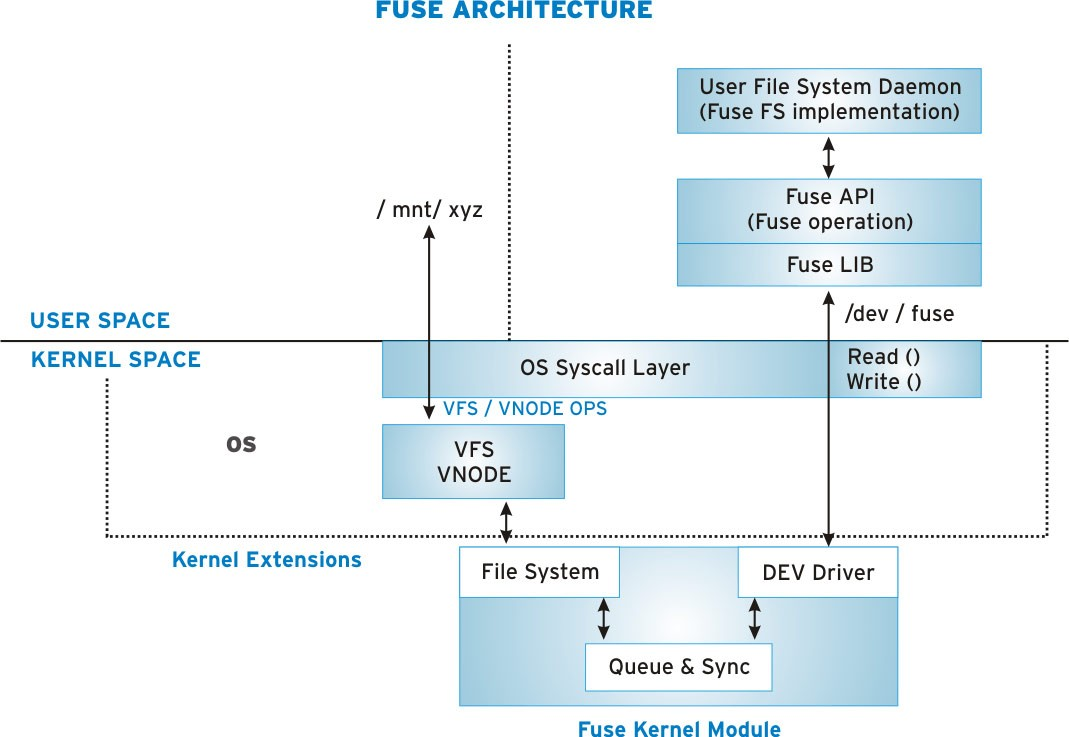
\includegraphics[scale=0.26]{img/fuse_arch.png}}
	
	\let\thefootnote\relax\footnotetext{Source: FUSE Kernel Operations, Vikas Gera, 2006}
	
\end{frame}

\subsection{Comparission between FUSE and kernel fs implementations}

%--- obrigado-------------------------------------%

\begin{frame}[plain]

  \begin{center}
    \Huge Questions?
  \end{center}

  \vspace{0.2in}

  \begin{center}
	Andre Petris Esteve - \texttt{andreesteve@gmail.com}\\
	Zhenlei Ji - \texttt{zhenlei.ji@gmail.com}
  \end{center}
\end{frame}

\end{document}
